\documentclass[12pt,a4paper]{article}
\usepackage[utf8]{inputenc}
\usepackage[spanish]{babel}
\usepackage{amsmath}
\usepackage{amsfonts}
\usepackage{amssymb}
\usepackage{makeidx}
\usepackage{graphicx}
\usepackage{lmodern}
\usepackage{kpfonts}
\usepackage{fourier}
\usepackage[left=2cm,right=2cm,top=2cm,bottom=2cm]{geometry}
\author{Rodriguez Lopez Francisco Javier}
\begin{document}

\begin{center}
\LARGE \textbf{Universidad Politecnica de la Zona Metropoilitana de Guadalajara\\}


\includegraphics[scale=1]{Upzmg6.png} 

\large \textbf{Arreglos de Amplificadores de potencia}\\
\vspace{2cm}
\large \textbf{Nombre:\\
Gúzman Vázquez Jaime Alan Yamil.\\
Ródriguez López Francisco Javier.\\
\vspace{0.5cm} Matricula:\\
18311861.\\
18311804.\\
\vspace{0.5cm} Carrera: Ingeniería en Mecatrónica.\\
\vspace{0.5cm} Materia: Sistemas Electrónicos de Interfaz.\\
\vspace{0.5cm} Curso: septiembre-noviembre del 2019.\\
\vspace{0.5cm} Docente: Morán Garabito Carlos Enrique.}


\vspace{3cm}
\small \textbf{07 de Noviembre del 2019}
\end{center}

\section{Introducción:}

Los amplificadores en el mundo de la potencia, son de muy amplia gama, asi tambien como sus arreglos, y de ayuda a la hora de transimitr tanto la corriente que se maneja en cualquier sistema, como el voltaje de traspaso. Los arreglos que se les pueda dar a estos, dada potencia de señales en las que es transmitido, son variados, y entre ellos el modo en que se les pueda utilizar, contando cada uno con caracteristicas peculiares, que te ayudan o complementan en la hora de tener que servir una mejor potencia y un mejor voltaje en sus terminales y de ello en sus conexiones, en las que sea acomodado\\

Ya sean estos, sumadores, restadores, algoritmicos, entre otros acomodos y arreglos, los cuales son objeto de estudio, para la buena sustitucion de algunos componentes que son remplazados por estos componentes y como estos, pueden llegar a un maximo y a un minimo de potencia requerida, en las conexiones que se esten usando y como se utilicen.  Dando un trabajo de rendimiento medio, o rendimiento maximo, en constancia de potencia y como esta puede ser utilizada con mayor eficiencia y sin conflictos de por medio.\\

Lo que se estara observando y explicando en esta practica, seran algunos de los arreglos que se les puede dar a los amplificadores operacionales, con el fin de poder comprender y analizar, como este componente, es de mucha ayuda, a la hora de ser un buen transmisor de voltaje, esto dado al recibimiento que se tiene en la amplitud de su uso, y como este es usado, en terminos mas exactos y factibles de comprender, ya sea pasando de una señal a otra, o conviertiendola en otro tipo de señal y onda, esto hecho por el arreglo que se tiene en ellos, y la buena colocacion de componentes, que hacen ver el buen uso de estos. Dentro de sus terminos, hay gran variedaad de ellos, en este reporte de practica se trato de ver la funcionalidad del LM741, ya que este nos deja tener una amplitud coloquial sin siquiera, tener que pasarlo a una tierra para que este cause fallas, o complicaciones que se puedan dar con otros amplificadores.\\



\section{Objetivo:}
Desarrollar por medio de OrCAD, la amplificacion de potencia dentro de arreglos.

\section{Material:}
\begin{itemize}
\item OrCAD 16.5.
\end{itemize}

\section{Procedimiento:}

\textbf{INVERSOR:\\}
Comenzaremos por explicar el amplificador operacional en su forma inversora, en donde por medio de un voltaje de entrada y una resistencia en configuración lazo llamada RF, ademas de una resistencia a la entrada llamada Rin  por donde entrara el voltaje y la corriente, debido a que el amplificador operacional no permite la entrada de corriente, la corriente  escapa por el resistor en configuración lazo, debido a esto se puede decir que la corriente de entrada es igual a la corriente del resistor en la salida, la configuración inversora se determina la pata de entrada que se seleccione la resistencia de lazo ya sea positiva o negativa.\\\\
Para calcular la amplificación que entregara el circuito se debe hacer un calculo simple de amplificación dividiendo la resistencia de referencia, la que esta en la configuración del lazo de forma negativa (debido a su configuración inversora) entre la resistencia que esta en la entrada del amplificador operacional, esto daría el resultado de la amplificación que se espera para la onda de salida.\\

\begin{center}
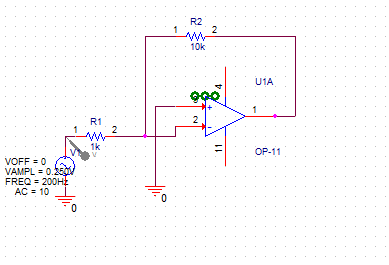
\includegraphics[width=11cm]{Simulaciones/inversor.png} 
\end{center}

$$G=\frac{-RF}{Rin}$$\\
donde G es la ganacia del circuito.\\
RF es la resistencia en lazo.\\
Rin es la resistencia en la entrada del operacional.
\\\\Donde en el caso del circuito simulado da una ganacia de -10 veces.\\
El esquematico se muestra en el apartado de resultados.\\\\

\textbf{NO INVERSOR:\\}
En el caso de el amplificador operacional en configuración inversora es el mismo principio que en el inversor, los únicos cambios que se mostraran en en este seria que las entradas el voltaje de entrada sera direccionando a la pata positiva mientras que la resistencia en forma de lazo sera configurado en la pata negativa con anclaje a tierra.\\
ademas de esto en los cálculos el único cambio que se realizara es que la resistencia de referencia RF no esta de forma negativa esta vez puesto que es un amplificación no inversora y quedaría de esta forma:\\
$$G= \frac{RF}{Rin}$$\\
donde G es la ganancia del circuito.\\
RF es la resistencia en lazo.\\
Rin es la resistencia en la entrada del operacional.\\
En donde el circuito simulado da una ganancia de 10 veces el voltaje\\

\begin{center}
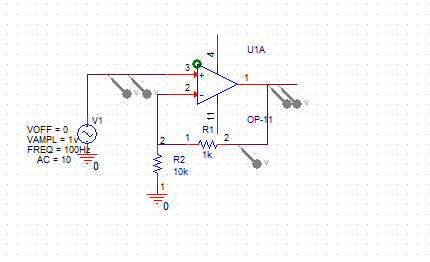
\includegraphics[width=10cm]{Simulaciones/noinver.png} 
\end{center}

\textbf{SUMADOR:\\}
El funcionamiento del circuito sumador seria el agregar tensión a la salida del amplificador operacional para poder amplificar cualquier entrada de voltaje y entregar una salida mucho mas grande esto en función de la ganancia que puede entregar en función de las resistencias que se tienen.\\
Esta configuración sigue los mismo principios que la no inversora solo que este caso se agregan 5 resistencias mas debido a que el sumador que se realizo es de 3 entradas y cada una necesitaría 2 resistencias de entrada ademas de la resistencia de referencia común de todas como se muestra en el diagrama en el apartado de resultados.\\\\
El principal uso de este amplificador operacion en esta configuracion seria el de sumas 2 o mas voltajes para entregar un unico voltaje de salida es decir la suma de todos los voltajes de entrada, el calculo de este, para calcular el voltaje de salida seria simplemente dividir cada voltaje entre su resistencia y sumarlos para entregar el resistor Rin como se muestra a continuacion:\\
$$Vout=(\frac{V1}{R1}+\frac{V2}{R2}+\frac{V3}{R3}....)$$\\
donde Vout es el voltaje de salida.\\
V1 es la fuente numero uno (así sucesivamente con cada fuente.)
R1 sera la resistencia del voltaje 1 (así sucesivamente con cada resistencia.)\\\\En el circuito simulado dio un voltaje de salida de 400mV
 Asi sucesivamente hasta entregar la suma de todas las entradas de voltaje, si se tiene el mismo valor de resistencia se sumara unicamente entonces el voltaje  unicamente para saber cuanto voltaje saldrá.\\nota: se deben realizar igualmente los cálculos de ganancia anteriormente explicados.\\
 
\begin{center}
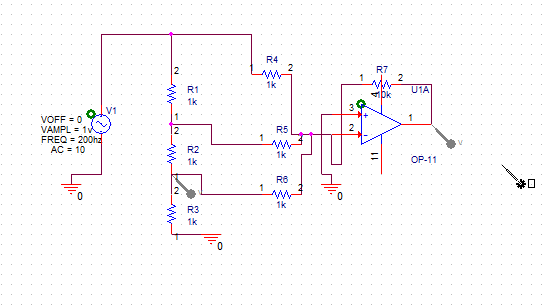
\includegraphics[width=10cm]{Simulaciones/suma.png} 
\end{center}
 
\textbf{RESTADOR:\\}
La configuración del tipo restador hace uso de una mezcla entre un amplificador inversor con uno no inversor, este resta una señal de la otra es decir la acción contraria que generaría el circuito sumador se aplica generalmente para eliminar el ruido que pueda contener una señal debido a cuestiones externas, esta configuración puede ser apreciada en el apartado de resultados en donde se muestra el diagrama del mismo ademas de la señal de salida que por supuesto entrega una señal menor de salida a la de entrada.\\\\
Los cálculos para esta serian los siguientes:\\\\ 

$$ Vout=V2(\frac{(R3+R1)R4}{(R4+R2)R1})-V1\frac{R3}{R1}$$\\
Donde Vout es el voltaje de salida\\
V2 seria el segundo voltaje.\\
V1 seria el primer voltaje .\\
R1,R2,R3... son las resistencias del circuito.\\ 
\\Los calculos de la simulacion dieron como resultado 100mv\\

\begin{center}
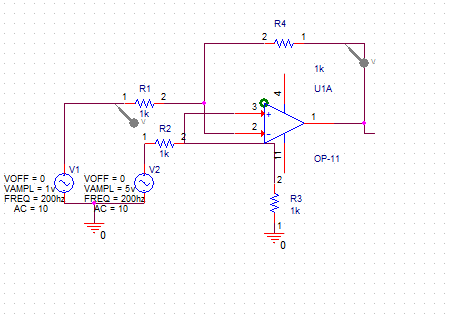
\includegraphics[width=10cm]{Simulaciones/res.png} 
\end{center}

\textbf{DAC:\\}
Esta configuracion del amplificador operacional se utiliza para convertir señales digitales a señales analogas en donde se coloca una linea con un switch y una resistencia de por medio para evidenciar cada bit, si se queiren 4 bit se ponen 4 lineas como lo es en este caso posteriormente se pasa la señal al amplificador operacional en donde se forma el cambio de voltaje permitiendo que la señal que parece un representa un bit se de mostrado un incremento o decremento en la señal, al final teniendo una onda senoidal que es reconstruida con los picos mas altos del voltaje interpretandose como una señal analoga.\\\\
para que  se logre realizar esta tarea es necesario el generar el calculo para saber que valor debe tener la resistencia en funcion de el maximo voltaje que en el caso de la señal digital serian 5v formando el 1 logico mientras que el 0 logico es formado por los 0 voltios esto se realiza calculando seria el numero de voltios 5v para el 1 logico entre el numero de bit que se desean de la siguiente forma:\\\\
$$RIND=\frac{1logico}{bit deseados}$$\\
donde RIND representa el valor de cada resistencia en la linea.\\
1logico serian los 5v.\\
bit deseado los bit que seran necesarios en el circuito.\\
En el caso de la simulación dio 1.25 ohm en cada resistencia.\\\\

\begin{center}
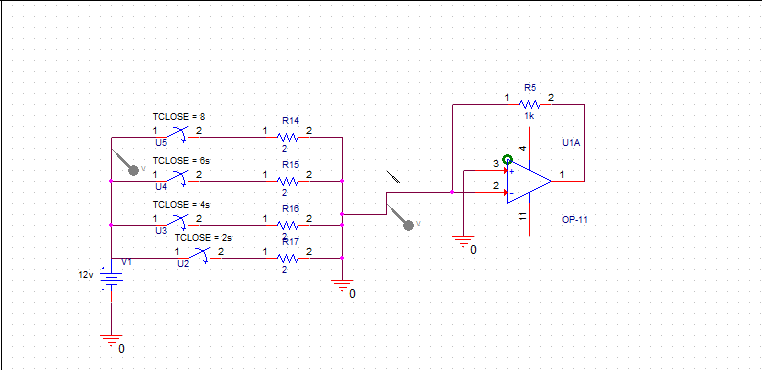
\includegraphics[width=10cm]{Simulaciones/DAC.png} 
\end{center}

\textbf{ADC:\\}
Este circuito toma la señal de 2 fuentes de voltaje y las compara en funcion de la otra enviando un 1 logico o un 0 logico dependiendo de la las fuentes y cual sea mayor la que esta conectada en la parte de el positivo de la entrada o la que esta en la entrada negativa de esta esto se va variando dependiendo de las resistencia que estan conectadas en serie que están divididas por solamente un switch estos para agrandar o aligerar la carga de ohms en el circuito permitiendo la comparación variable de los mismos, para esta configuracion de conversion se necesita de igual forma el calculo anterior para determinar la resistencia de cada circuito y en funcion de eso poner para que represente cada bit.\\

\begin{center}
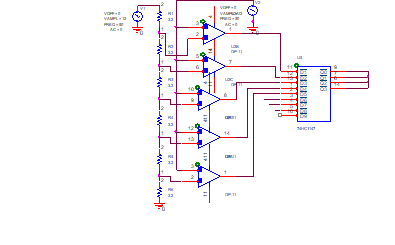
\includegraphics[width=10cm]{Simulaciones/ADC.png} 
\end{center}

\section{Resultados:}

Los resultados generados se estaran, viendo y explicando, la generacion de señales y la generacion de ondas, por medio de los arreglos requeridos.

\begin{center}
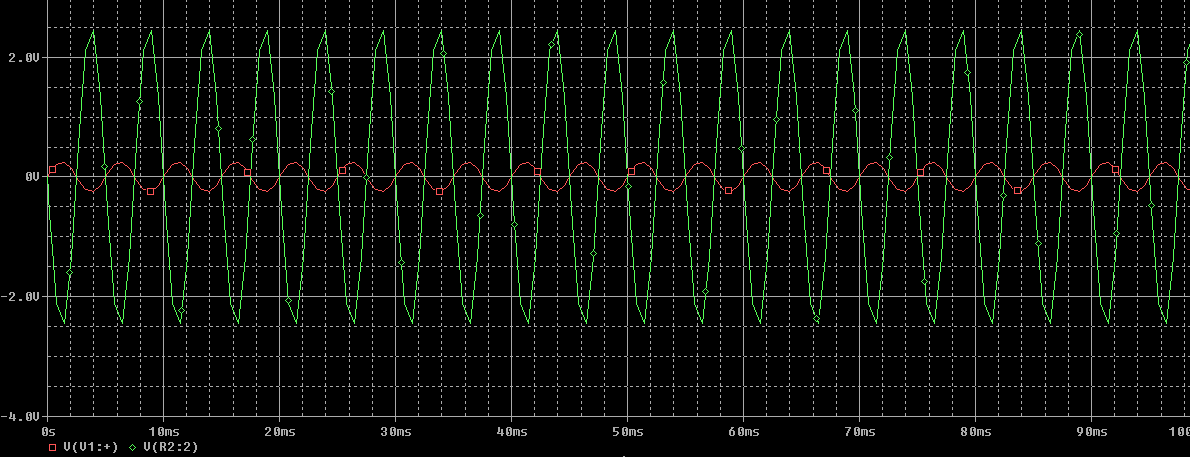
\includegraphics[width=10cm]{Simulaciones/inverso.png} 
\end{center}

El resultado de las conexiones para el inversor,son estas, notese que dan de esa manera una mas grande y otra onda mas corta, por la generacion de potencia, y el acomodo de la amplificacion dada las señales que recibe el circuito esquematico, comotal.\\
Ahora se estara viendo, el no inversor, para ver como actua el circuot y las ondas en este caso.

\begin{center}
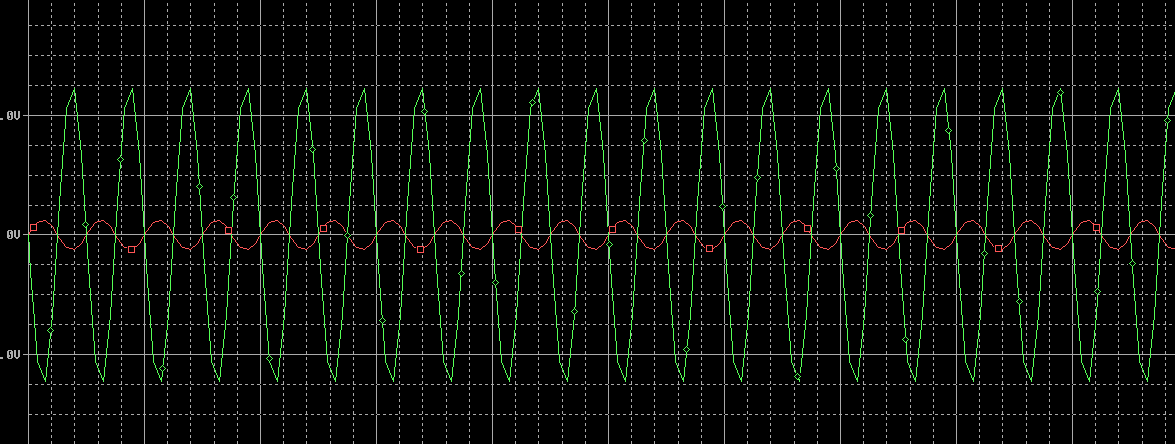
\includegraphics[width=10cm]{Simulaciones/noinvers.png} 
\end{center}

La del no inversor, en este caso, las señales son en constante muy similare, pero con la diferencia de invertir, no invierte, sino que su estado esta constante, en una señal mas fuerte en subida, pero mas pequeña en entrada, asi pues cumpliendo la funcion de no inversor, para la generacion de las señales.

\begin{center}
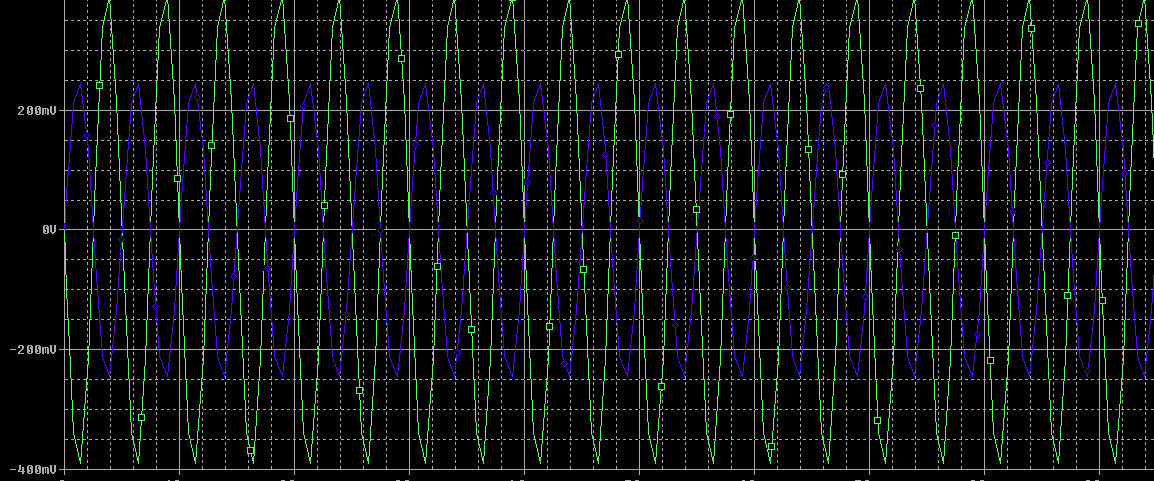
\includegraphics[width=10cm]{Simulaciones/sumat.png} 
\end{center}

En este caso, el sumador en casos de amplificacion, genera estos resultados, obteniendo esto, por la señal que recibe a la entrada y el acomodo que este tiene, para dar y generar esas señales de onda, siendo esto, de gran ayuda, para a visualizacion de l arreglo sumador en constancia a amplificacion.

\begin{center}
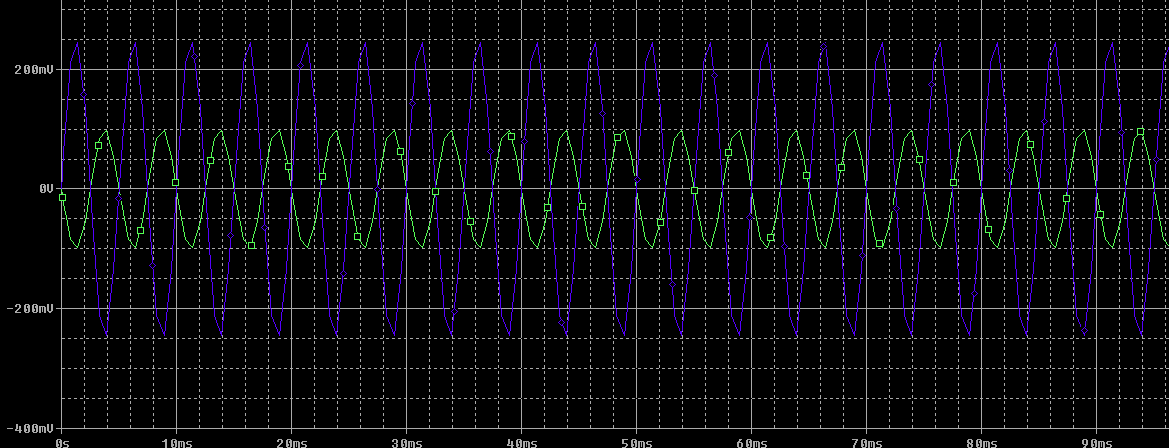
\includegraphics[width=10cm]{Simulaciones/rest.png} 
\end{center}

Como se ve en el nombre, el esquematico, del restador, es el inverso, al del sumador, ya que este su generacion de ondas es menor, en constancia al acomodo que se le de a la amplificacion, desde la entrada recibida, hasta la generacion de salida, dejando ver la amplifiacion y generacion de ondas en acomodo restador.

Ën el caso, del DAC y ADC, la generacion de ondas, son en escalera en el caso del DAC, convirtiendo y generando una señal digital en una analogica, dejandoo ver entre ondas senoidales, que se convierten en un tiempo estimado, en ondas de escalera, que se comunican entre los parametrso de tiempo en los que son establecidos, el cambio de onda a onda (Digital a Analogica).\\\
En el caso, del ADC, convirtiendo una señal Analogica a Digital, este es pura en una onda a escalera, ya que las pautas del tiempo dados los parametrso, en los que se este trabajando, y con que voltaje se este trabajando, el acomodo del esquematico, hara su trabajo, que cada amplificador, y su arreglo en estancia de bits, se centrara en enviar una señal y convertirla en el parametro de tiempo establecido, genereando un voltaje en cada salida de voltaje, en escalera.\\

\begin{tabular}{|c|c|c|}
\hline
	codigo binario  & DAC & ADC\\
\hline
	0000 & 0v & 220v-200v\\
\hline
	0001 & 1.25v & 190v\\
\hline
	0010 & 2.5v & 180v\\
\hline
	0011 & 2.8432v & 170v\\
\hline
	0100 & 3.73v & 160v\\
\hline
	0101 & 3.8297 & 140v\\
\hline
	0110 & 3.985v & 130v\\
\hline
	0111 & 4.04v & 120v\\
\hline
	1000 & 4.72918v & 110v\\
\hline
	1001 & 4.72936v & 90v\\
\hline
	1010 & 4.72974v & 80v\\
\hline
	1011 & 4.72992v & 70v\\
\hline
	1100 & 4.7358v & 60v\\
\hline
	1101 & 4.73076v & 40v\\
\hline
	1110 & 4.73113v & 30v\\
\hline
    1111 & 4.73131v & 20v\\
\hline
\end{tabular}\\


Nota: No se muestran las imagenes de las ondas, ya que el software proporcionado, no nos da la configuracion, para poner parametros de tiempo, por lo que la muestra de las ondas, queda mostrada al docente.\\

\textbf{\Large Conclusion:}\\

\textbf{Jaime Gúzman}:\\
Las simulaciones que se realizaron son de gran importancia puesto que son todas en base a la utilización de amplificadores operacionales, ya sea el amplificar una señal, el restarle intesidad  a esta o el comparar dos entradas de voltaje para generar una respuesta y envia una señal son cuestiones que el amplificador operacional puede hacer, ademas de poder hacer muchas mas configuraciones.\\ estas aplicaciones son muy relevantes, ejemplificando esto tenemos las dos ultimas simulaciones que se realizan convertidores de señales analogicas a señales digitales y viceversa, esto es algo que practicamente se usa  en todo tipo de diferentes partes de la electronica, o de igual forma la amplificacion de señales es muy utilizada cuando las señales recividas son muy pequeñas o demasiado debiles, esto es de igual forma muy importante para cualquier ambito de la industria.\\

\textbf{Francisco Rodriguez:}\\
Los arreglos, de los amplificadores, pueden dar en su conmstancia, muchas de las herramientas, que se puedan ver en un futuro, en materias, de mayor control, y mejor sentir en el disparo, de la señales que este genere, en este caso,sumando, restando, o incluso convirtiendo, una señal a otra, dados los acomodos que este tenga, y como estan siendo utilizados.\\
Para su mayir fuerza y requerimiento en paso a las ondas generadas, y xomo estos, pueden ser de gran aprendizaje, en generacion, a las ondas que su señal pueda conmutar y de que manera, convenciendo de que los arreglos, dados los amplificadores y el tipo de amplificador, nos pueden ser de ayuda en otras practicas, y teorias mas complejas.\\

\textbf{\Large Referencias:}\\

Op Amps and Linear Integrated, Circuits: Theory and Aplication, Libro de James M. Flore 2004, Theory of circuits Analog-Digital.\\

Carlos Enrique Moran Garabito, Sistemas Electronicos de Interfaz, Curso: Sep-Dic 2019 c, Arreglos de amplificadores de potencia.


\end{document}